\section{Concurrency Errors}

\subsection{Sequential Consistency}

\begin{itemize}
    \item Instructions are executed by the order they appear in the program.
    \item Memory behaves as a shared array. (Reads and writes are effective immediately)
    \item This is naturally true for a sequential program, but it is not true for concurrent program!
\end{itemize}

\subsection{How to see correct states?}

First we go the maximum we can go in one side, until we find a precedence. Next we advance the minimum from the other side until our precedence is fulfilled.


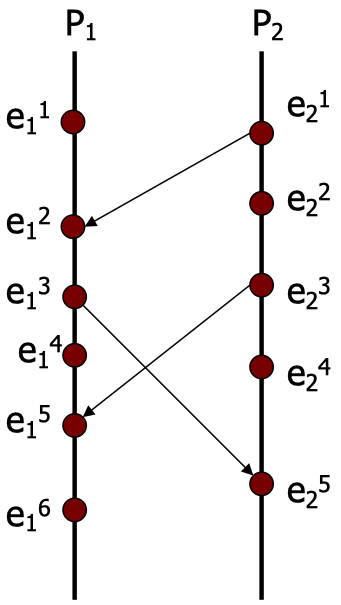
\includegraphics[width=0.1\textwidth]{ConcurrencyErrors/gRAPH.png}

\subsection{Common Concurrency Errors}

\begin{itemize}
    \item Data Races (atomicity violations)
    \item Ordering violation
    \item Unintended sharing
    \item High-level atomicity violations
    \item Deadlocks
    \item Livelocks
\end{itemize}

\subsection{Data Race Detection}

\subsubsection{Static Program Analysis}
Advantages:
\begin{itemize}
    \item Reason about all inputs/interleavings
    \item No run-time overhead
    \item Adapt well-understood static-analysis techniques
    \item Possibly with annotations to document concurrency invariants
\end{itemize}

Disadvantages:

\begin{itemize}
    \item Tools produce "false positives" and/or "false negatives"
    \item May be slow, require program annotations
    \item May be hard to interpret results
    \item May not scale to large or complex programs
\end{itemize}


\subsubsection{Dynamic Program Analysis}

Advantages:
\begin{itemize}
    \item \textbf{Soundness} - Every actual data race is reported
    \item \textbf{Completeness} - All reported warnings are actually races (avoid "False Positives")
\end{itemize}

Disadvantages:

\begin{itemize}
    \item Run-time overhead (5-20x for best tools)
    \item Memory overhead for analysis state
    \item Reason only about observed executions
\end{itemize}

Types of algorithms:

\begin{itemize}
    \item Lock-set Algorithm
    \item Happens-Before
    \item Noise-Injection
\end{itemize}

\textbf{Happens-Before} : Defines a partial order for events in a set of concurrent threads. We can stablish a happen-before if we have locks (lock in one thread, unlock in order thread over the same lock).

\textbf{Lock-set Algorithm}\par
Two data structs (LockHeld(x) , LockSet(x)) \par
When thread 't' acquires lock 'l' = $LocksHeld(t) = LocksHeld(t) \cup {l}$ \par
When thread 't' releases lock 'l' = $LocksHeld(t) = LocksHeld(t) \setminus {t}$\par
When thread 't' accesses location 'x' = $LocksSet(x) = LocksHeld(t) \cap LocksSet(t)$\par
"Data race" warning if Lockset(x) becomes empty. \par
Locks Held start empty and LockSet Start with all locks.\par
No warnings is equivalent to no data races on the current execution, but wanings does not imply data race.\par


\subsubsection{High Level Data Races}

\textbf{View Analysis} is composed by every variable read and written in a block of code.

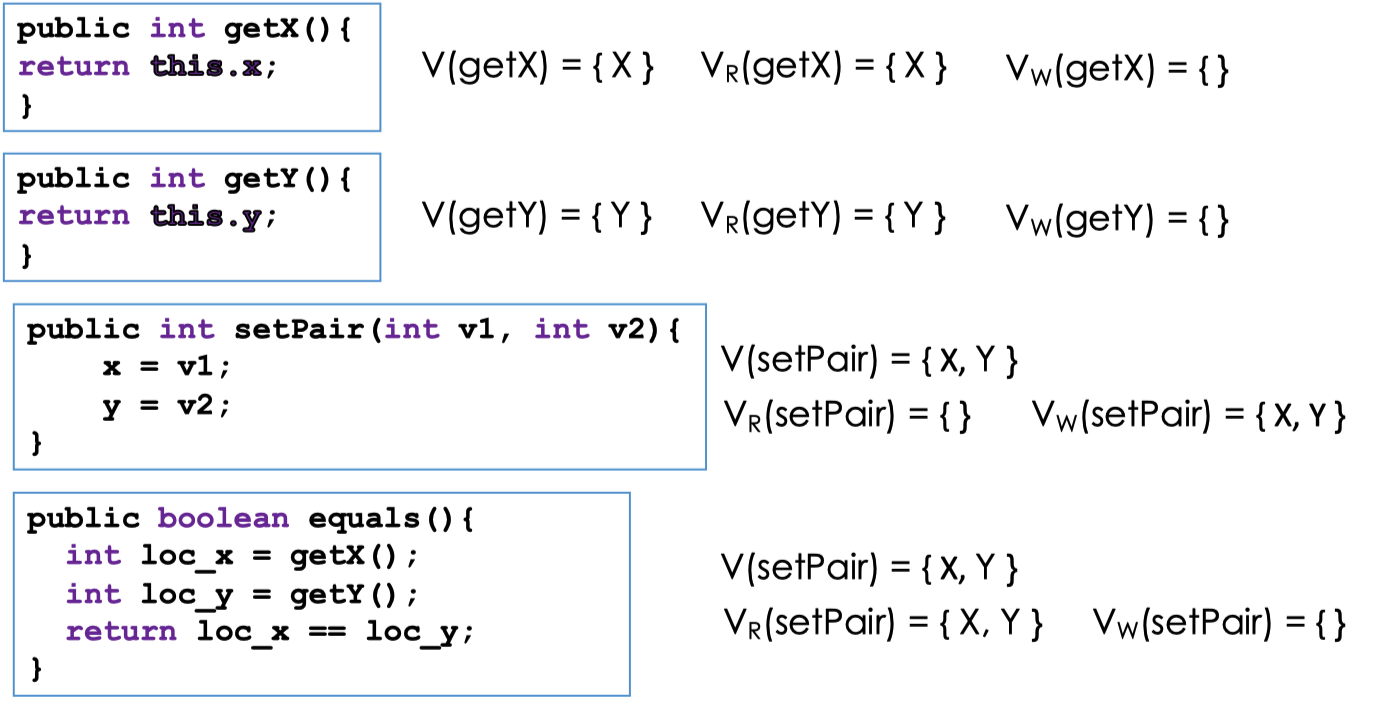
\includegraphics[width=0.20\textwidth]{ConcurrencyErrors/view.png}

\textbf{Casual Dependencies Graph}= Data Dependencies + Control Dependencies.\par

There is a direct correlation between a read variable 'x' and a written variable 'y' if in the dependency graph D there is a path from 'x' to 'y'\par
There is a Common Correlation between read variable 'x' and 'y' if in a dependency graph d, there is a write variable 'z' such that: 'z != x' and 'z != y' and there are paths from 'x' to 'z' and from 'y' to 'z'

\textbf{Test for HLDR}

T1 runs V1 = {A,B,C} and V2 = {A,B,C,D}\par
T2 runs V3 = {A,B,E} and V2 = {B,C,F}\par
IS THERE A HLDR?\par

V2 is maximal in T1\par
$V2 \cap V3 = {A,B}$\par
$V2 \cap V4 = {B,C}$\par
${A,B} \subseteq {B,C} or {B,C} \subseteq {A,B}$ No!\par
Common-Correlation(A,C)?\par
 - YES! high Level Data Race \par
 - No! No High Level Data Race

\subsection{Deadlock Detection}

A set of two or more processes are deadlocked if:\par
\begin{itemize}
    \item They are blocked (i.e in the waiting state)
    \item Each is holding a resource
    \item Each is waiting to acquire a resource held by another process in the set.
\end{itemize}[]

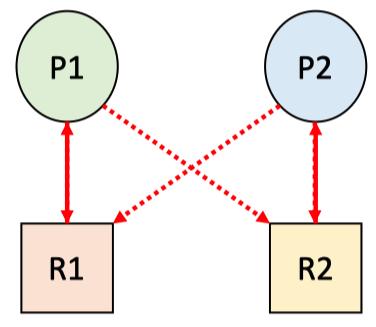
\includegraphics[width=0.1\textwidth]{ConcurrencyErrors/graphdeadlock.png}

\textbf{Condicions Necessary for Deadlock}\par
\begin{itemize}
    \item \textbf{mutual Exclusion} only one process can use a resource at a time
    \item \textbf{hold and wait} a process holding at leadt one resource is waiting to acquire additional resources which are currently held by other processes.
    \item \textbf{no preemption} a resource can only be released voluntarily by the process holding it.
    \item \textbf{cirular wait} a cycle of processses requests exists ($P_0 -> P_1 -> P_2 -> ... -> P_{n-1} -> P_0$)
\end{itemize}

\subsection{Resource Allocation Graph}

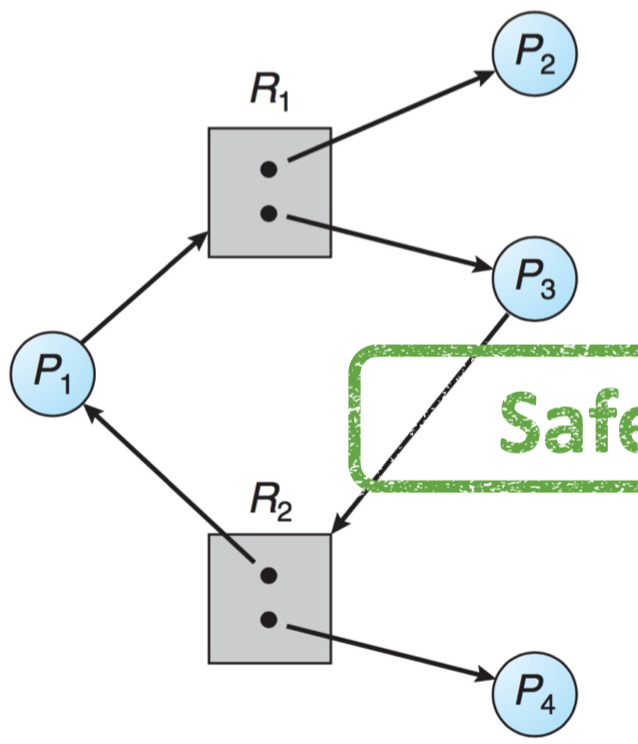
\includegraphics[width=0.1\textwidth]{ConcurrencyErrors/ressourcegraph.png}

If a graph contains no cycles -> No deadlock \par
If a graph contains a cycle -> \par
-if onyly one instace per resource type, then deadlock\par
- if serveral instaces per resouce type, possibility of deadlock.

\subsection{How to Deal with deadlocks}

\begin{itemize}
    \item Deadlock prevention
    \item Deadlock avoidance
    \item Deadlock detection and recovery
    \item Ignore the issue!
\end{itemize}

\subsection{Deadlock Prevention}

Restrict the way requests can be made...\par
\textbf{Mutual Exclusion}\par
\textbf{Hold and Wait}\par
-must guarantee what whenever a process requests a resource, it does not hold any other resources.\par
-require process to request and allocate all its resources before it begins execution.\par
-low resource utilization; starvation possible\par
\textbf{No Preemption} \par
- if a process that is holding some resources requests another resource that cannot be immedialy allocated to it, then all resources currently being held are released.\par
- Preempted resources are added to the list of resources for which the process is waiting.\par
 process will be restarted only when it can regain its old resources, as well as the new ones that it is requesting.\par
 \textbf{Circular Wait}\par
 - impose a total ordering of all resources types, and require that each process requests reources in an increasing order of enumeration.
 
 \subsection{Deadlock Avoidance}
 
 Requires that the system has some additional a priori information available.\par
 - Requires that each process declares the maximum number of resources of each type that it may need\par
 - The deadlock-avoidance algorithm dynamically examines the resource-allocation state to ensure that there can never be a circular-wait condition.
 - Resource-allocation state is defined by the number of available and allocated resources, and the maximum demands of the processes.\par
 
 \textbf{System is in safe state} if there exists a sequence of ALL the processes in the system such that for each Pi, the resources that Pi can be satisfied by currently available resource + resource's held by all the Pj, with j < i \par
 
 If a system is in safe state -> no deadlocks\par
 If a system is in unsafe state -> possibility of deadlock\par
 Avoidance -> ensures that a system will never enter an unsafe state.
 
 
\subsection{Avoidance Algorithms}

Single instance of a resource type, use a resource-allocation graph\par
Multiple instances of a resource type, use the bankers algorithm\par

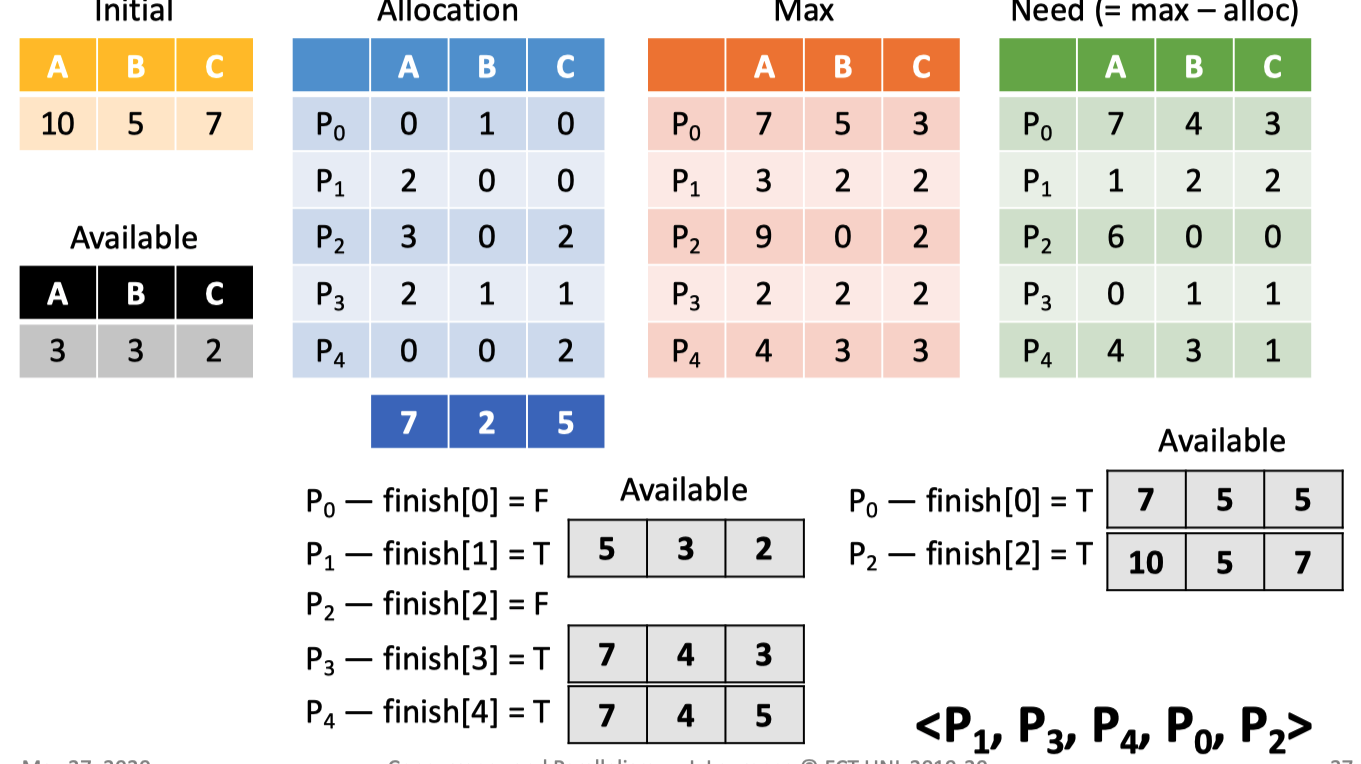
\includegraphics[width=0.20\textwidth]{ConcurrencyErrors/bankers.png}